\subsection{The purpose of storing data directly as raw file}
In the comprehensive compilation acquired during the recent field excursion, an
array of invaluable data was meticulously gathered, meticulously chronicled, and
thoughtfully analyzed. Specifically, our focus gravitated towards the
operational activities conducted within the radar center situated in the Nha Be
district. Operating at the pinnacle of technological advancement, the radar
center diligently executes periodic scans of the atmospheric conditions,
facilitating the meticulous documentation and exportation of a SIGMET file,
which serves as a repository encapsulating a myriad of meteorological phenomena
and atmospheric dynamics.

The SIGMET file, serving as the quintessential embodiment of scientific rigor
and methodological precision, meticulously records a plethora of critical
parameters and meteorological variables. Among the salient features meticulously
delineated within this archival masterpiece are the discerning metrics of
reflectivity and wind radial velocity. Reflectivity, a fundamental metric in
radar meteorology, is an indispensable parameter delineating the intensity of
electromagnetic waves returned to the radar antenna from various atmospheric
particles, thereby furnishing crucial insights into the spatial distribution and
intensity of precipitation within the monitored region. Furthermore, the wind
radial velocity, an elemental component in meteorological analysis, delineates
the rate and direction of atmospheric motion along the radial axis relative to
the radar antenna. These metrics serve as a vital tool in elucidating the
intricate dynamics of atmospheric circulation, enabling meteorologists to
decipher prevailing wind patterns, identify regions of convective activity, and
forecast the trajectory of severe weather phenomena with enhanced accuracy and
precision.

Yet, amidst the effervescent tapestry of meteorological data acquisition and
analysis, a conundrum of paramount importance arises: the optimization of data
storage and retrieval mechanisms. It is within this crucible of inquiry that the
proposition to store meteorological results directly within the file repository
assumes a mantle of significance, heralding a paradigm shift in data management
practices.

Indeed, the inherent multidimensionality of meteorological data, encapsulated
within its tripartite tensor structure, underscores the imperative for a
streamlined approach to data storage and retrieval. By eschewing aggregation and
denormalization techniques, we advocate for a direct integration of results
within the archival framework, thereby fortifying the foundations of data
integrity and computational efficiency.

Moreover, the proposition to leverage the existing ETL (Extract, Transform,
Load) system developed by Vaisala, as utilized by our esteemed National Center
for Hydrometeorological Forecasting, emerges as a beacon of pragmatism and
resourcefulness. In a landscape fraught with technological complexities and
budgetary constraints, the utilization of pre-existing infrastructure represents
a judicious allocation of resources, affording seamless integration and
interoperability across disparate data management platforms.

In summation, the decision to store meteorological data directly within the file
repository, without resorting to further aggregation techniques, emerges as a
testament to both pragmatism and foresight. By embracing this approach, we not
only enhance the accessibility and usability of meteorological datasets but also
lay the groundwork for a new era of scientific inquiry and meteorological
prognostication, fortified by the pillars of technological innovation and
methodological rigor.


\subsection{Extracting data from each of the radar center}
We have authored a script, albeit not yet integrated into the operational
system, designed to facilitate the redirection of the SIGMET (Significant
Meteorological Information) file from the data center to our preconfigured
Storage Server.

Presently, the script is implemented in Python to ensure platform-agnosticism.
Accompanied by a concise setup script, it will be poised for execution on the
radar center's machinery.

MinIO has been employed as an unstructured data repository owing to its
compatibility with the S3 (Simple Storage Service) protocol. As the system
matures in the distant future, transitioning to AWS S3 should be
straightforward. The underlying logic and API for interfacing with the storage
infrastructure remain largely invariant during such a migration.

\begin{lstlisting}[language=Python, caption={Part of the script for uploading data to Storage}]
file_path = pathlib.Path(args.filename)

s3_client = boto3.client( "s3", endpoint_url=os.getenv("S3_HOSTNAME"),
    aws_access_key_id=os.getenv("S3_ACCESS_KEY_ID"),
    aws_secret_access_key=os.getenv("S3_SECRET_ACCESS_KEY"), ) _ =
    s3_client.upload_file(file_path, os.getenv("S3_BUCKET"),
    generate_new_name(file_path.name))
\end{lstlisting}

\setlength{\emergencystretch}{3em} % provides additional stretching to avoid
underfull hboxes

Currently, we follow a designated nomenclature for naming data files of the
RADAR objects: \texttt{<year><month><day>T<hour><minute><second>}. This system
enhances the speed of data retrieval for specific times of the day. Utilizing S3
Prefix filtering, we can efficiently select multiple data points within a time
frame that may vary from a second to an entire year.

For instance, to query data for a specific day (e.g., 2024-03-15), utilizing the
UNIX path wildcard, we can express our query as:

\begin{lstlisting}[language=sh]
ls 20240315T*
\end{lstlisting}

Analogously, the same query can be executed using the \texttt{boto3} library in
Python:

\begin{lstlisting}[language=Python, caption={Querying data in 2024-03-15}]
def query_with_wildcard(bucket_name): s3_client = boto3.client('s3')
    
    response = s3_client.list_objects_v2( Bucket='nha-be-radar',
        Prefix='20240315T' )
        
    return [obj['Key'] for obj in response['Contents']]
\end{lstlisting}

Moreover, although our naming convention deviates somewhat from the ISO-8601
standard for timestamp representation, the inclusion of the letter \textbf{T}
aids in swiftly identifying datetime components within the naming structure.

One limitation of this naming convention is its inability to support wildcard
querying for a central time component. Consider the scenario necessitating data
retrieval for a specific hour daily. Utilizing the UNIX wildcard, this can be
depicted as:

% Correct use of the lstlisting environment
\begin{lstlisting}[language=sh]
ls 202403*T09*
\end{lstlisting}

The utilization of an internal wildcard here implies the absence of an efficient
mechanism for querying such objects presently. The current recourse involves
maximal prefixing (e.g., \texttt{Prefix=202403}), followed by subsequent
filtering in Python.

\subsection{Data Explorer}
Besides S3-compatible API for accessing the storage, our solution also provides
some alternative ways for preview the data storage. This can be used for manual
intervention (in case of failure), or simply for the radar center's operators to
preview.

First, there is an online explorer that can be access from the web browser. As
you can see from Figure \ref{fig:minio-home}, the web UI is very user-friendly
and easy-to-use. With the use of IAM (shorts for Identity and Access Management)
and \textbf{Policies}, the admin user of our entire system can restrict what a
tenant (or a radar center) can see and what should be hidden.

\begin{figure}[H]
    \centering
    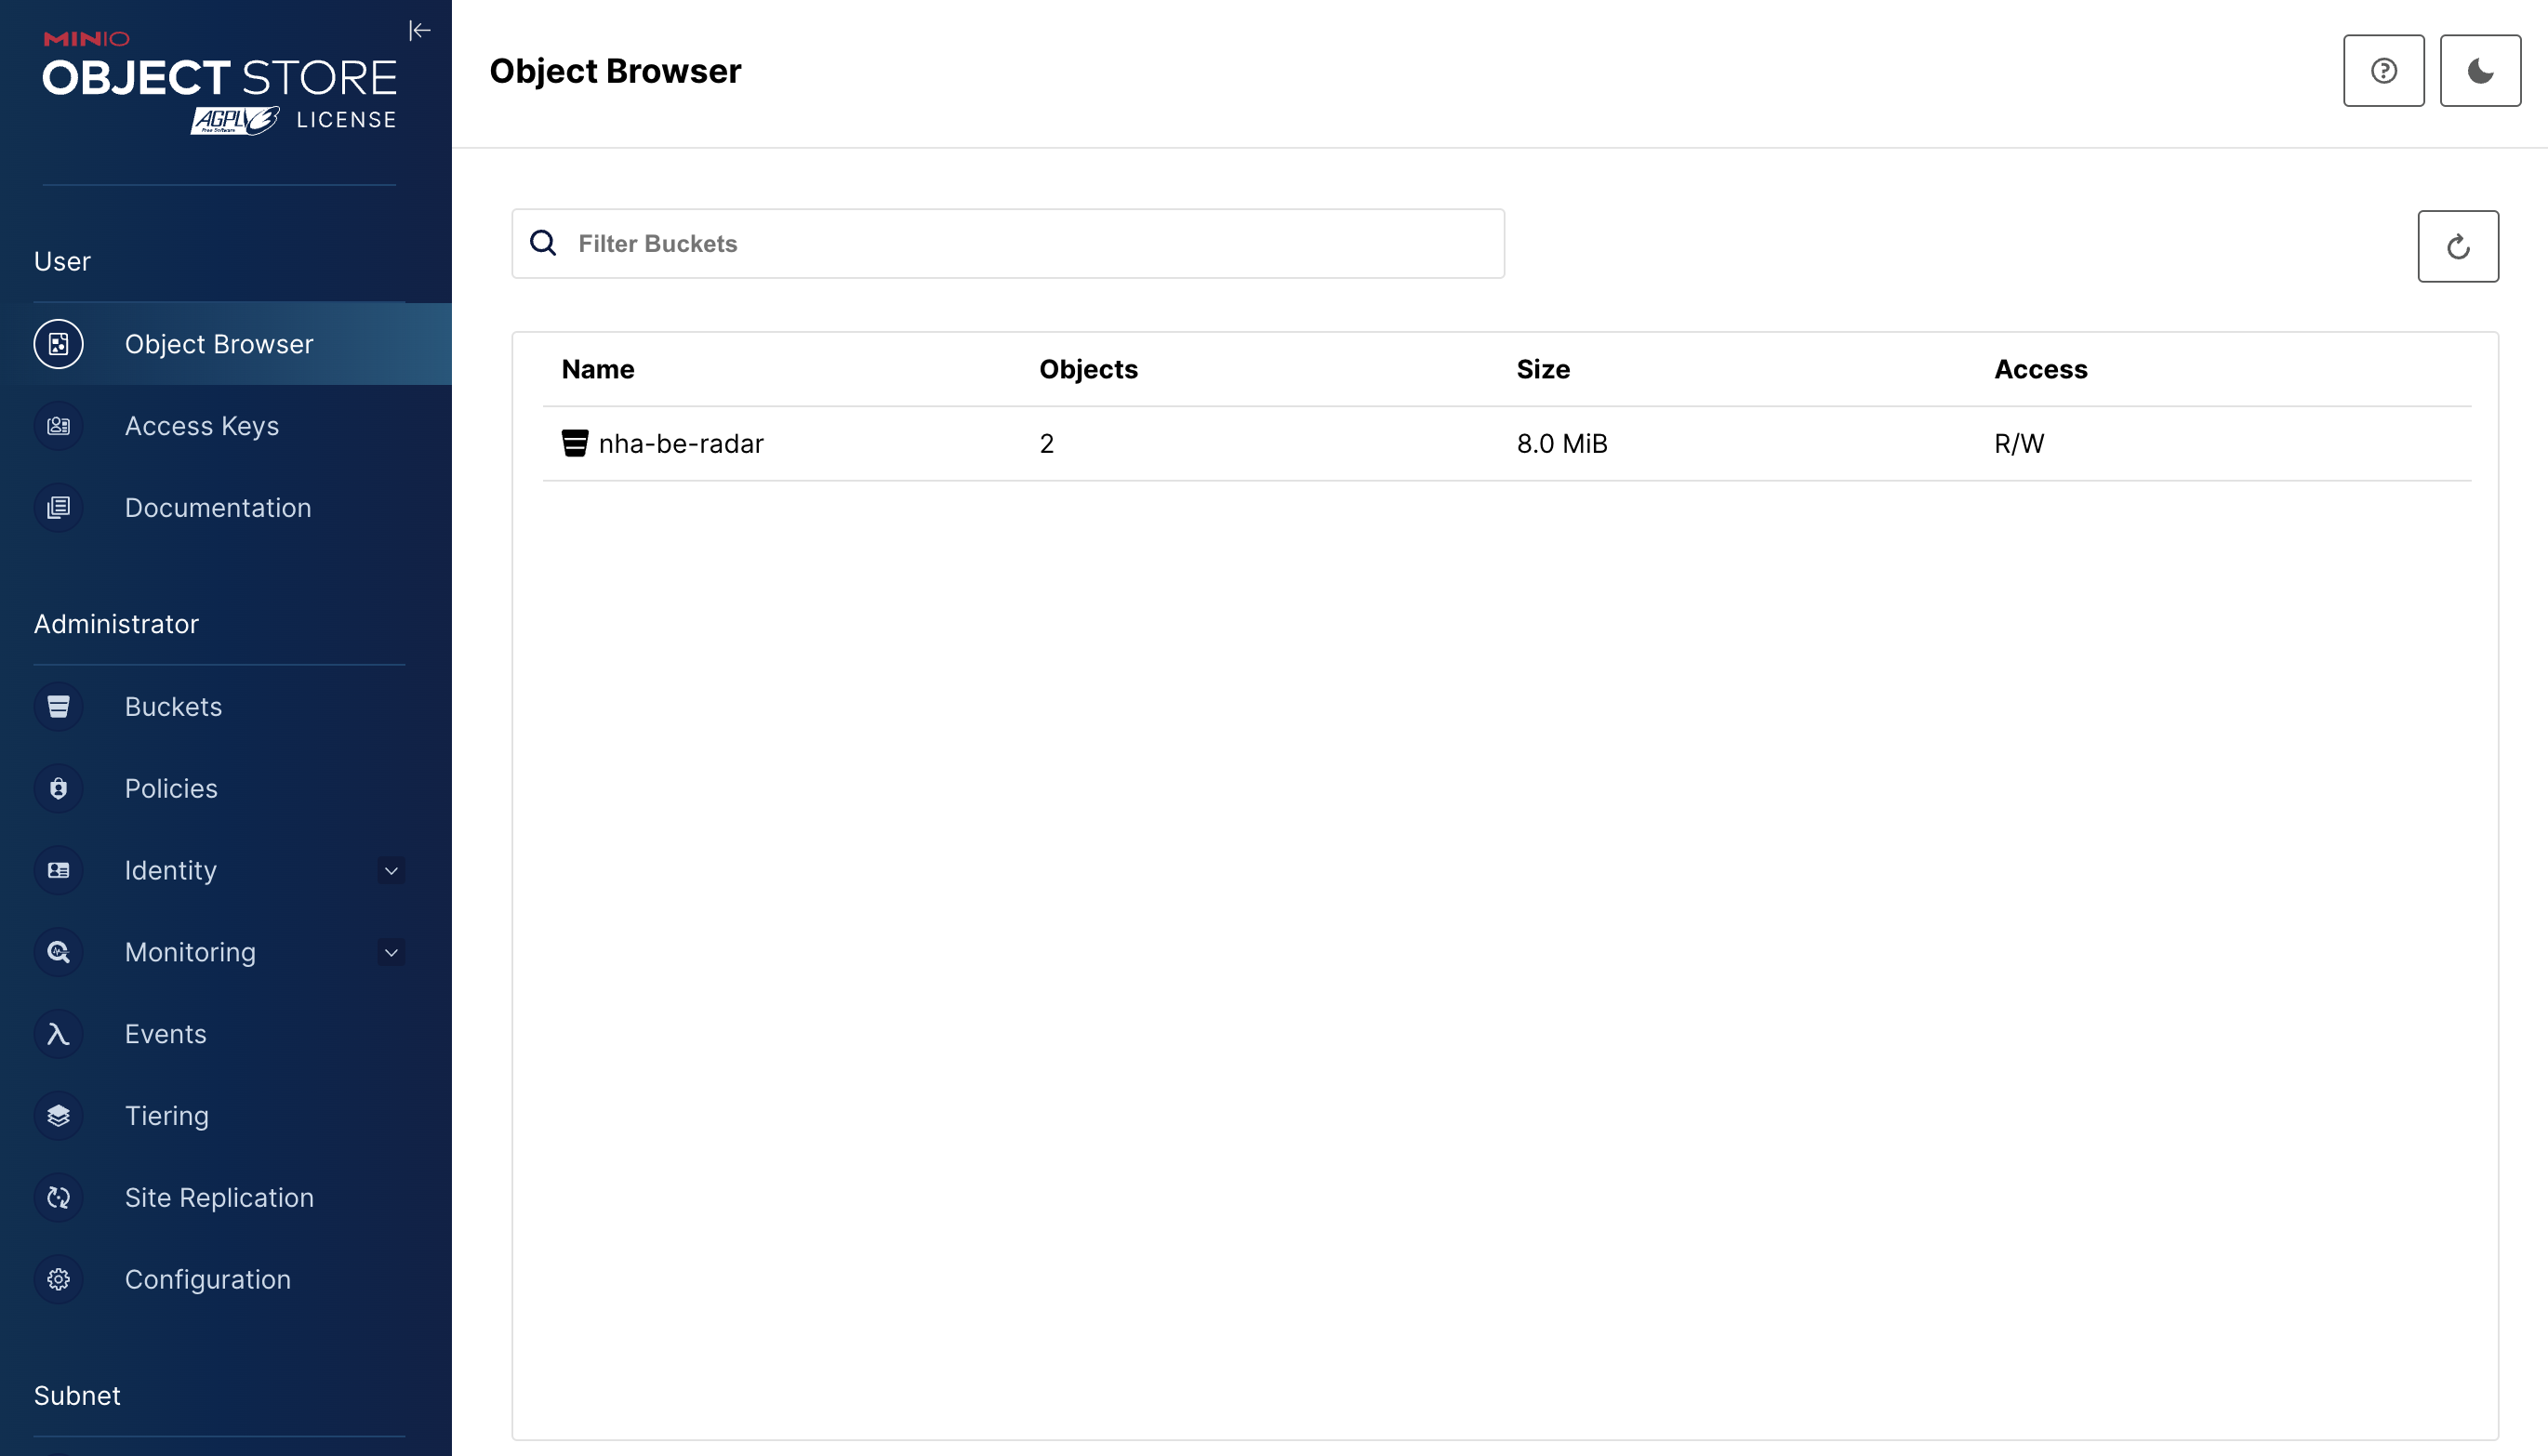
\includegraphics[width=0.8\linewidth]{Images/4.3-datastore/minio-bucket.png}
    \vspace{1em}
    \caption{MinIO web interface provides a clear and intuitive way to explore the storage}
    \label{fig:minio-home}
\end{figure}

Currently, as of the time of writing, our system has been self-hosted on a small
Raspberry Pi server. The explorer has been set up with necessary load balancing,
DNS and SSL/TLS registering correctly. Anyone that has been given proper
permissions can visit \url{https://explorer.meteor-flow.com/} to see the server
running. Figure \ref{fig:minio-files} shows some of the files that our team has
prepared beforehand.

\begin{figure}[H]
    \centering
    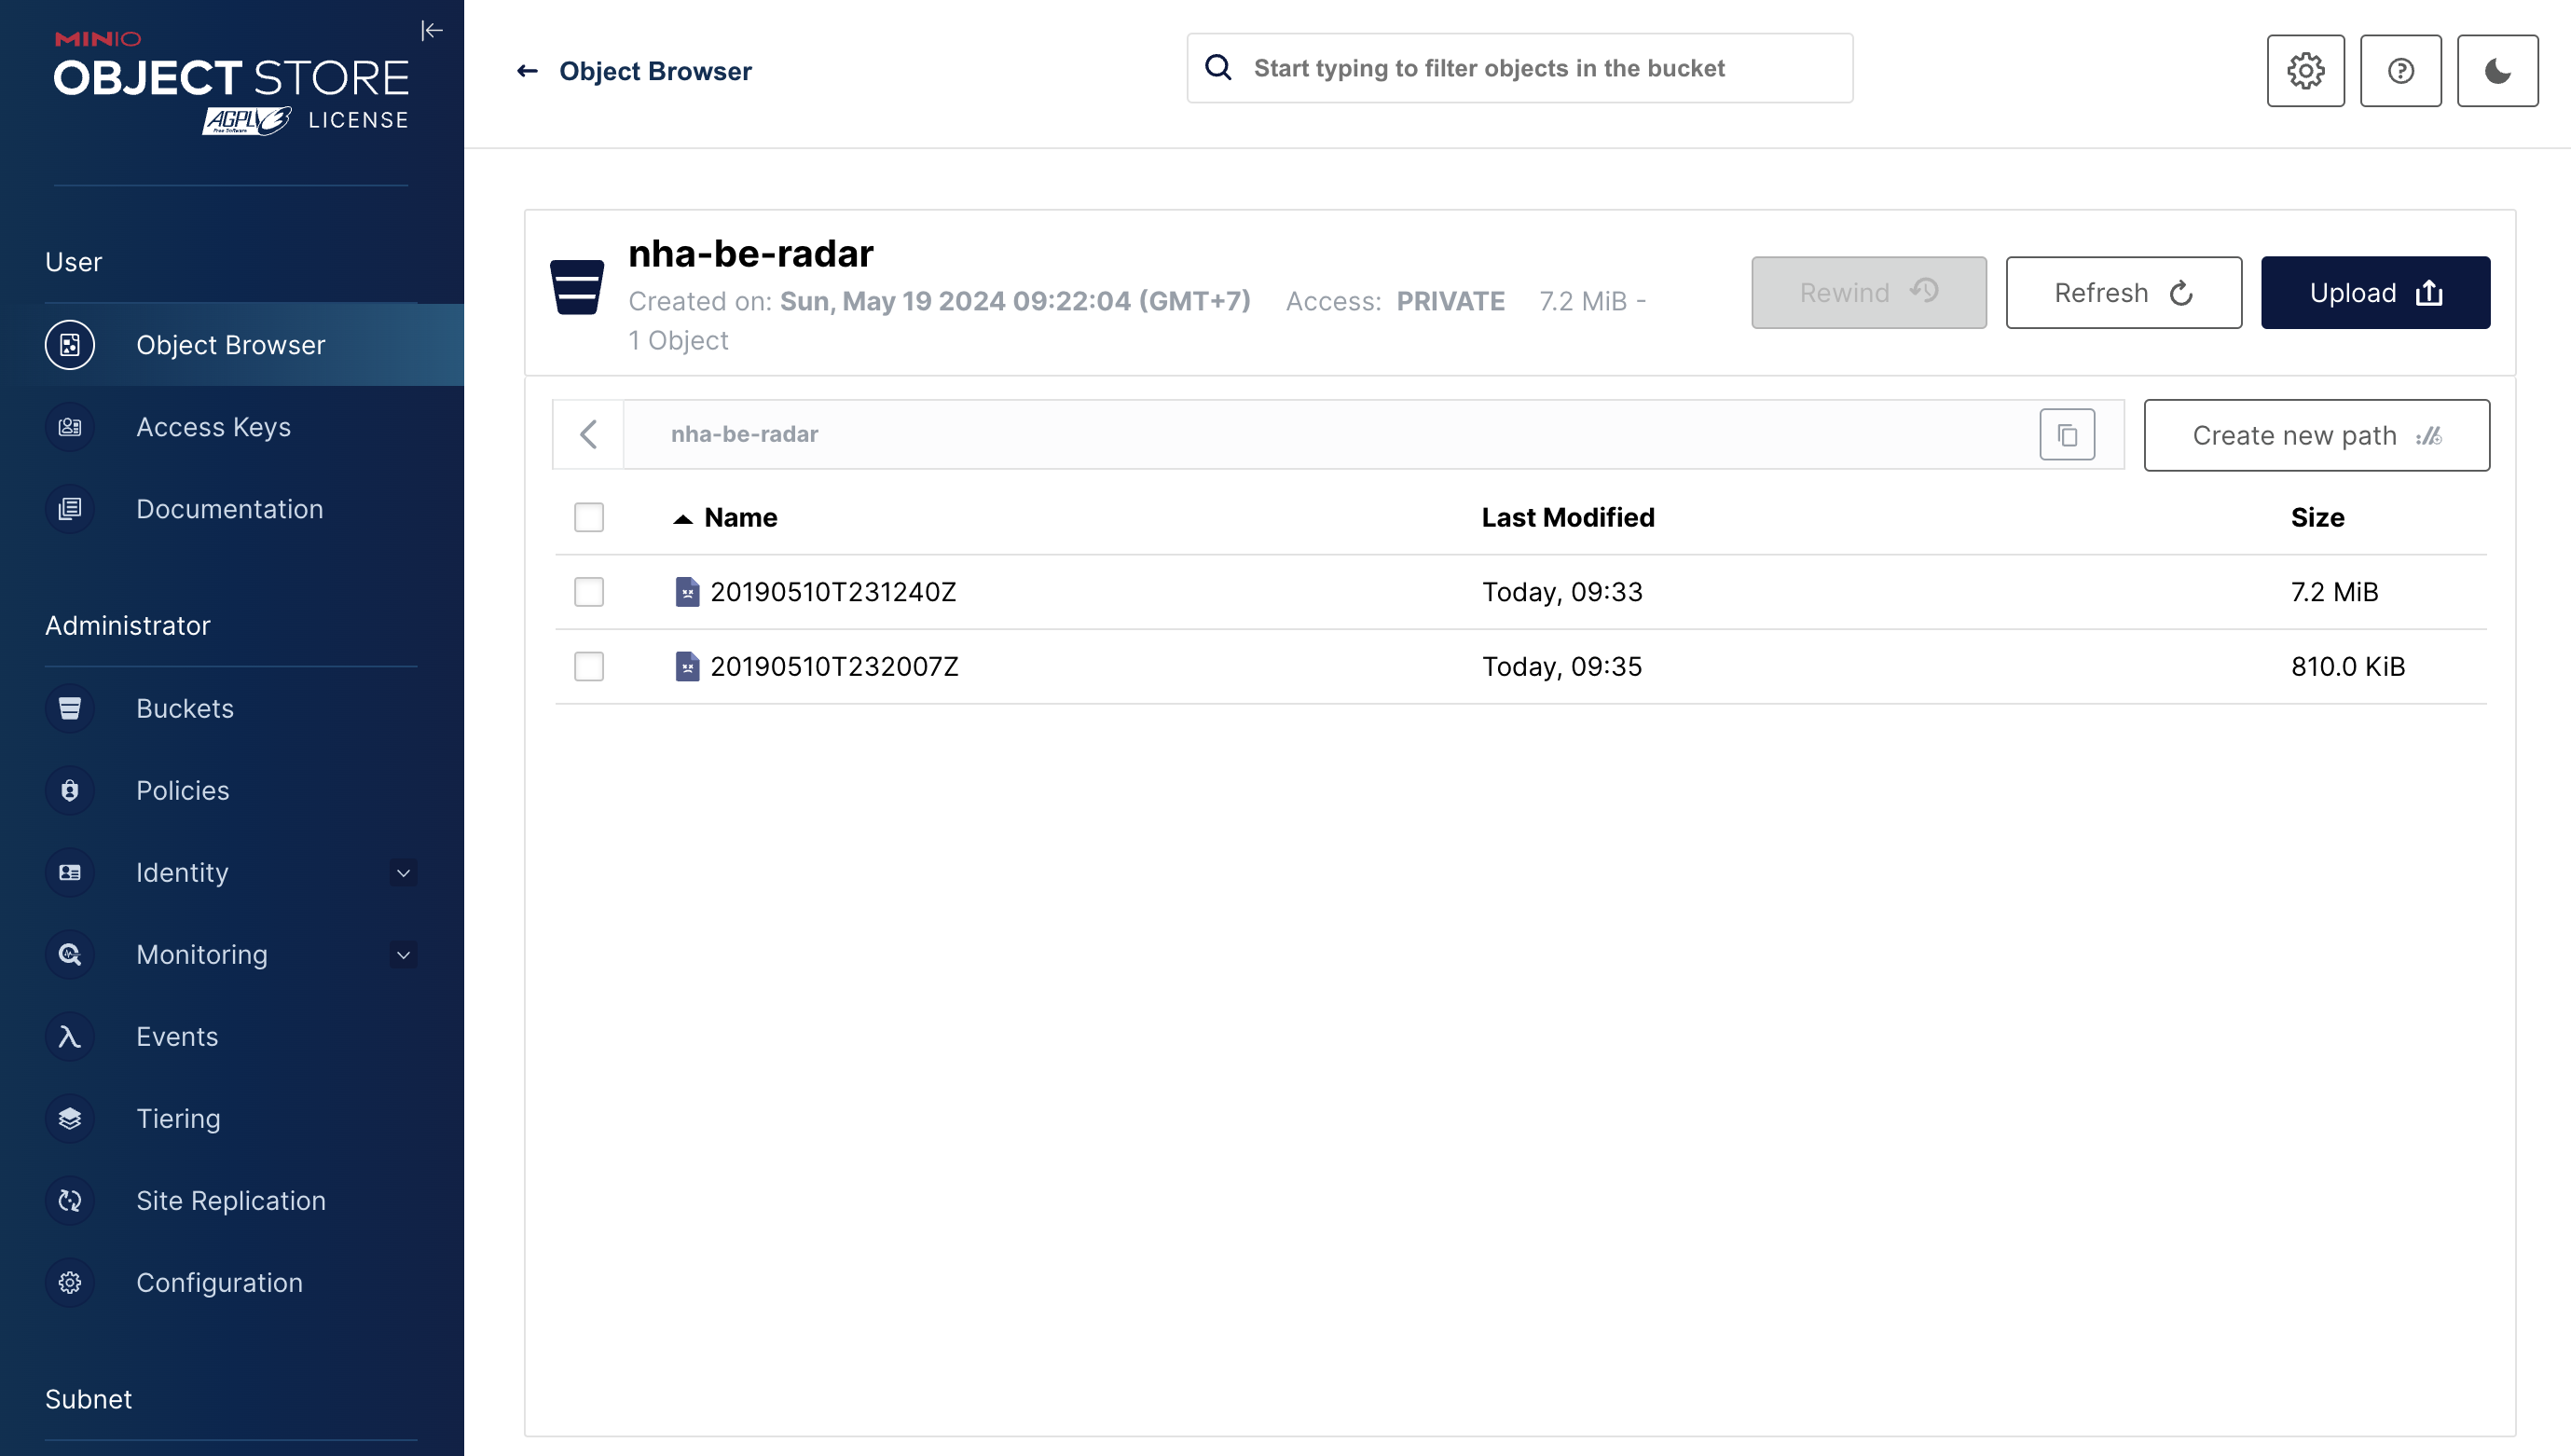
\includegraphics[width=0.8\linewidth]{Images/4.3-datastore/minio-files.png}
    \vspace{1em}
    \caption{Some radar files are currently being stored on the storage}
    \label{fig:minio-files}
\end{figure}


Not stopping at that, our system can also work with any other S3-compatible
client. One notable example of this is Cyberduck. In the future, our team can
research for more compatible protocols, such as FTP or SFTP.

\begin{figure}[H]
    \centering
    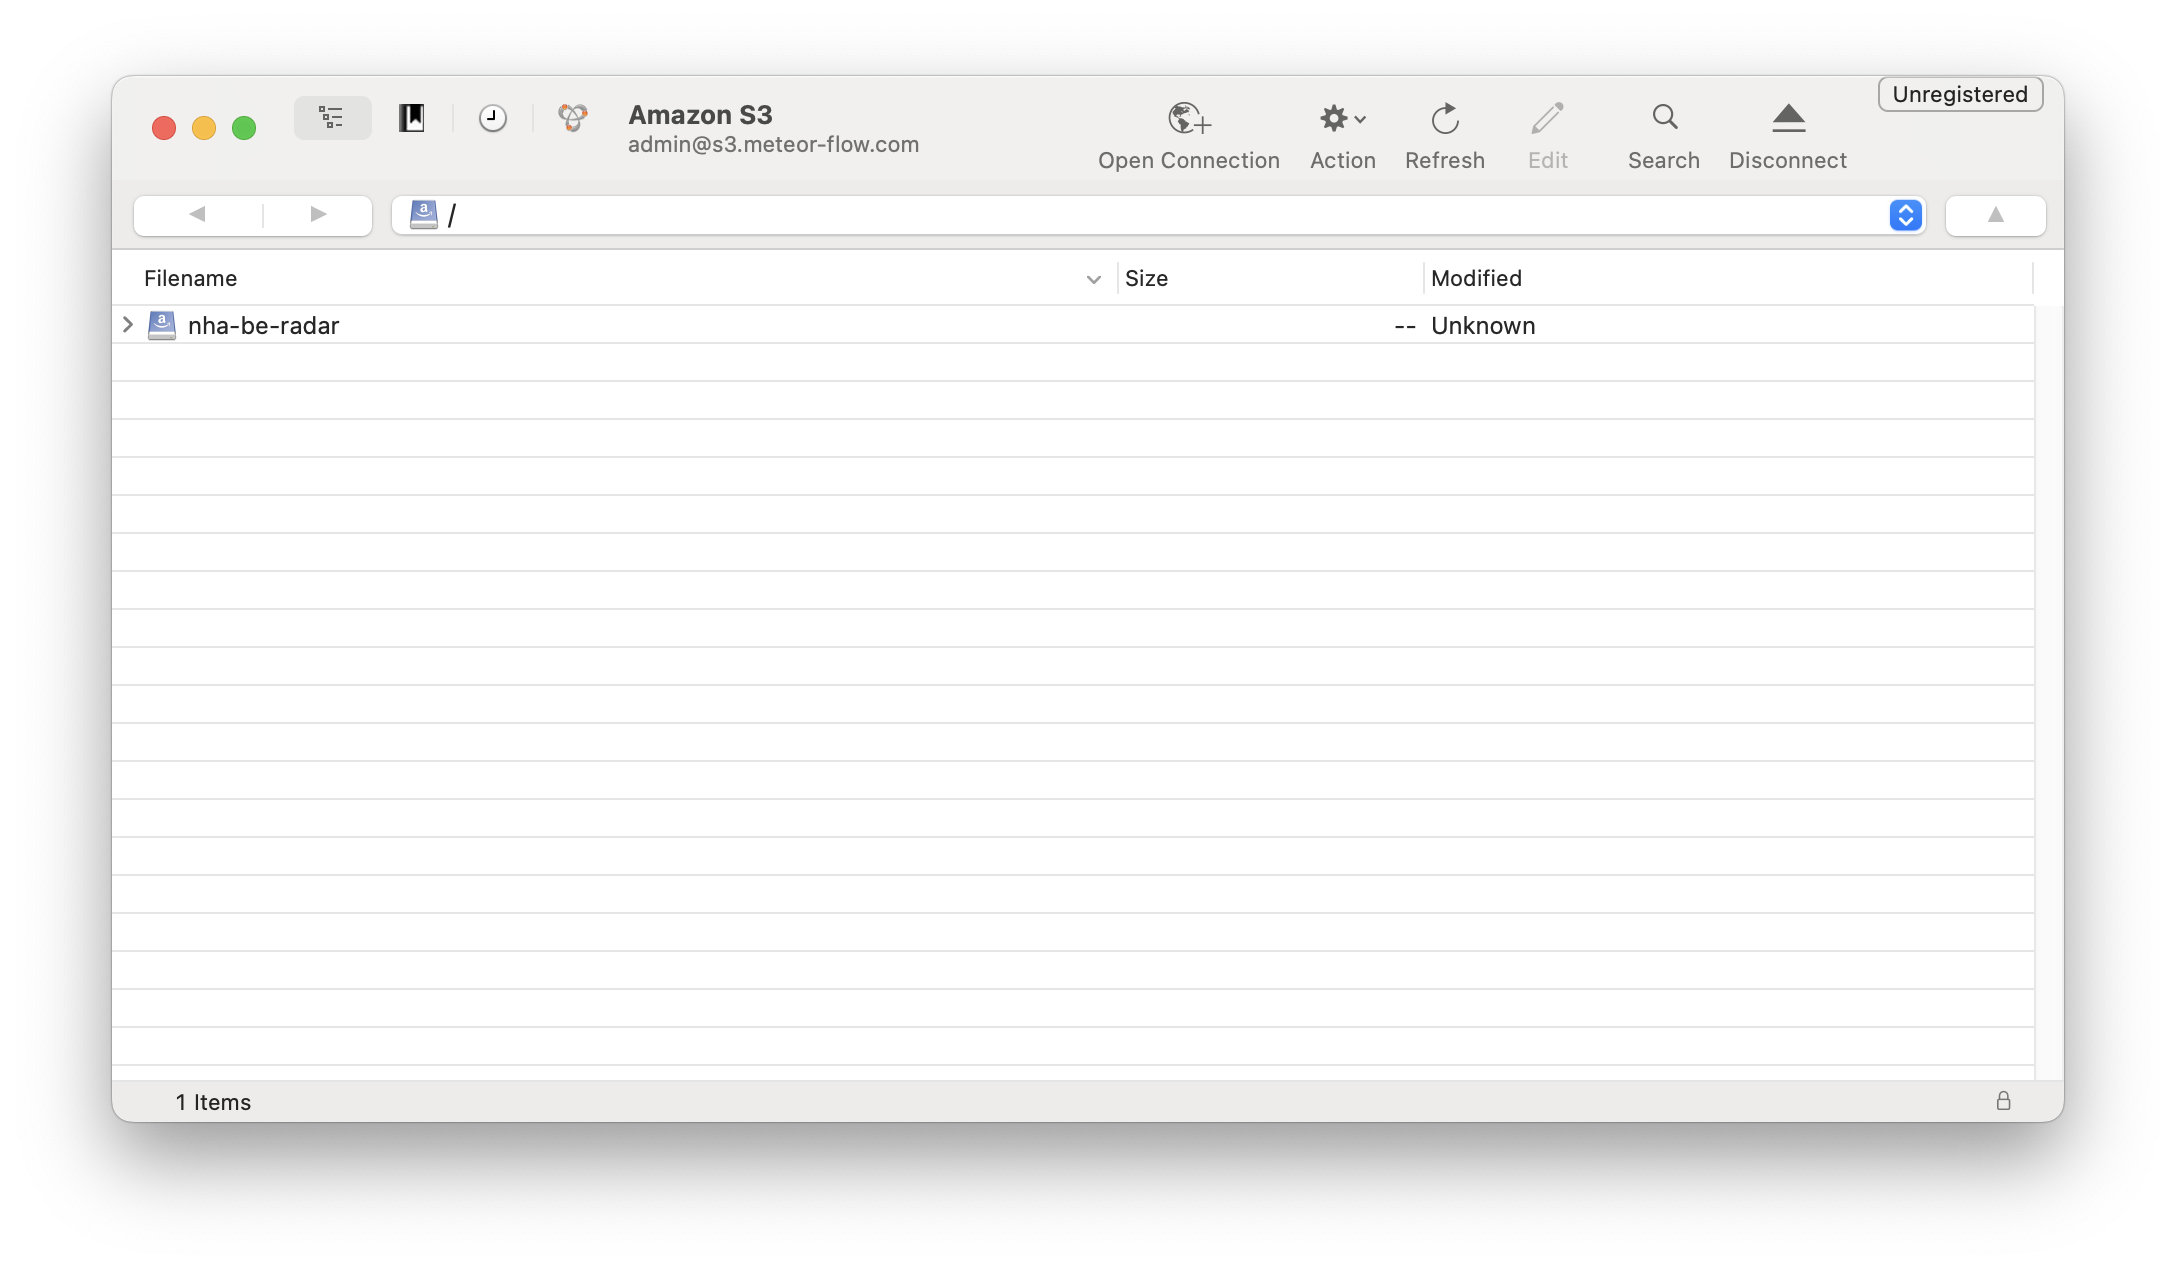
\includegraphics[width=0.6\linewidth]{Images/4.3-datastore/s3-client.png}
    \vspace{1em}
    \caption{Using Cyberduck to view data on the platform}
    \label{fig:s3-client}
\end{figure}
